\documentclass[]{dsadokumentation}

% Extra packages / definitions
\usepackage{amssymb}
\usepackage{amsthm}
\usepackage{algorithm}
\usepackage[noend]{algpseudocode}
\usepackage{wrapfig}



% Bibliography
\addbibresource{kurs4.2.bib}

% Custom Commands / definitions
\setcounter{chapter}{1}
\newcommand\myacademy{Wolfsberg 2022}


\begin{document}

\tableofcontents

\kurs{Die Theorie der Information}{Wie aus Daten Bilder werden}{example-image-a}

\section{Eigenwertproblem}
\sectionauthor{Lara Müller, Chuyang Wang}

\subsection{Definitionen}\label{k4.2.eigen.def}

Ein Eigenvektor ist der Vektor, welcher nach Anwendung einer Matrix immer auf einem Vielfachen von sich selbst liegt.
Formal werden die Eigenvektoren einer quadratischen Matrix $A \in \mathbb{R}^{x \times x}$ definiert als $\vec{v} \in \mathbb{R}^{x}, \vec{v} \neq \vec{0}$, mit denen $A \cdot \vec{v} = \lambda \cdot \vec{v}$ erfüllt ist. Man nennt das Skalar $\lambda$ den zu $\vec{v}$ zugehörigen Eigenwert.

Durch Äquivalenzumformung erhält man

\begin{equation}
  \label{k4.2.eigen.def.lgs}
  \begin{aligned}
     &                 & A \cdot \vec{v}               & = \lambda \cdot \vec{v}   &                                 & \\
     & \Leftrightarrow & A \cdot \vec{v}               & = \lambda E \cdot \vec{v} & \text{mit } \vec{v} = E\vec{v}  & \\
     & \Leftrightarrow & (A - \lambda E) \cdot \vec{v} & = 0                       &                                 & \\
     & \Leftrightarrow & B\vec{x}                      & = 0  \quad \quad          & \text{mit } B = (A - \lambda E) & \\
  \end{aligned}
\end{equation}

Die \textit{Determinante} einer Matrix ist ein skalarer Wert, welche die Eigenschaft dieser Matrix beschreibt. Dieses lineare Gleichungssystem \cref{k4.2.eigen.def.lgs} hat erst dann nicht-triviale Lösungen ($\vec{x} = 0$), wenn die Determinante von $B$ gleich $0$ ist. Also gilt $\det (B) = \det (A - \lambda E) = 0$.

Bei dem Eigenwertproblem gilt es, diese Vektoren sowie die zugehörigen Eigenwerte zu finden.


\subsection{Das charakteristische Polynom}

Im Allgemeinen wird das charakteristische Polynom definiert als $\chi_A (\lambda) = \det(A - \lambda E)$. Aus \cref{k4.2.eigen.def} folgt, dass man die Nullstellen dieses Polynoms finden muss, um den Eigenwert zu berechnen.

Betrachtet man nun beispielsweise das Problem in 2D. Sei $A = \begin{pmatrix}
    a & b \\
    c & d
  \end{pmatrix}$, so gilt

\begin{equation}
  \label{k4.2.eigen.charac.2d}
  \begin{aligned}
    0
     & = \chi_A (\lambda)                              \\
     & = \det(A - \lambda E)                           \\
     & = \det \begin{pmatrix}
                a - \lambda & b         \\
                c           & d-\lambda
              \end{pmatrix}                  \\
     & = (a - \lambda) \cdot (d - \lambda) - c \cdot b
  \end{aligned}
\end{equation}

Eine allgemeine Lösung für \cref{k4.2.eigen.charac.2d} kann dann mithilfe der pq-Formel berechnet werden:

\begin{equation}
  \begin{aligned}
    \lambda = \frac{a+d}{2} \pm \sqrt{\Big(\frac{(a+d)}{2}\Big)^2-ad+cb}
  \end{aligned}
\end{equation}


\subsection{Power Iteration}\label{k4.2.eigen.powerit}

Für $2 \times 2$ Matrizen lässt sich das Eigenwertproblem relativ gut lösen, da es eine allgemeine Formel (vgl. pq-Formel / abc-Formel) für das charakteristische Polynom existiert. Ab dem 5. Grad wird es jedoch unmöglich, eine allgemeine Formel herzuleiten \parencite{k4.2.ramond}. % Abel Ruffini Theorem
Mit dem Power-Iteration-Algorithmus versucht man, eine Annäherung an den höchsten Eigenwert zu berechnen. Der iterative Algorithmus wählt am Anfang einen willkürlichen Wert für $b_0 \in \mathbb{R}^n$. Bei jeder Iteration aktualisiert man diesen Vektor $b$ wie folgt:

\begin{equation}
  \begin{aligned}
    b_{k+1} = \frac{Ab_k}{\left\lVert Ab_k \right\rVert }
  \end{aligned}
\end{equation}

Nach ausreichenden Iterationen kann man den größten Eigenwert $\lambda$ berechnen, indem die Gleichung $B b_{k} = \lambda b_{k}$ nach $\lambda$ auflöst wird.


\subsection{Anwendungen}

Eigenwerte und Eigenvektoren sind wichtige Werkzeuge für viele mathematische Rechnungen und Beweise. Ein Beispiel dafür ist die Drehung durch eine Matrix: Wenn die Matrix $A$ eine Drehung um einen bestimmten Winkel beschreibt, dann ist der Eigenvektor die Drehachse, da seine Richtung durch die Drehung nicht verändert wird.

\section{Cox's Theorem}
\sectionauthor{Mara Germann, Patricia Hackl}
Wie berechnet man die Wahrscheinlichkeit eines Ereignisses, dem ein anderes Ereignis zugrunde liegt? Um diese Frage zu beantworten, bedarf es der Wahrscheinlichkeitsrechnung. Das Cox's Theorem ist die logische Grundlage für diese.


Beim Cox's Theorem wird die Wahrscheinlichkeitsrechnung aus  der Logik hergeleitet. Im Grenzfall für absolute Sicherheit für das Eintreten beziehungsweise Nichteintreten von Ereignissen geht die Wahrscheinlichkeitsrechnung in wahr/falsch Aussagen über. Mit Cox's Theorem entsteht eine in sich konsistente (einheitliche) Theorie für die Wahrscheinlichkeitsrechnung.
Aus dem Cox's Theorem lässt sich herleiten, dass man Wahrscheinlichkeiten als Grad der Plausibilität interpretieren kann. Wir werden später sehen, dass die Plausibilität der Wahrscheinlichkeit entspricht.
Das Cox's Theorem beruht auf 3 Axiomen, die die Begründung der Bayes'schen Wahrscheinlichkeitsrechnung sind.


\begin{itemize}
  \item[(1.)] Der \textbf{Grad der Plausibilität} eines Ereignisses $\{b|a\}$ wird als \textbf {reelle Zahl} dargestellt. Für hohe Plausibilitäten werden hohe Zahlenwerte gewählt. Dies ermöglicht den \textbf {universellen} Vergleich voneinander unabhängiger Plausibilitäten.

  \item[(2.)] Sinnvolle Ergebnisse werden unter qualitativem Miteinbezug des \textbf {Verstandes} und durch logische Schlussfolgerungen erzielt.
  \item[(3.)] Es müssen \textbf {alle }verfügbaren Informationen miteinbezogen werden. An die Schlussfolgerungen wird die Anforderung der \textbf {Konsistenz }gestellt, sodass alle Sätze, die gleiches Wissen vermitteln auf gleiche Plausibilitäten hinführen müssen.
\end{itemize}

Aus den Axiomen ergeben sich die Produktregel und die Summenregel für Wahrscheinlichkeiten, wobei $A$, $B$ und $C$ drei Ereignisse sind.

\subparagraph{Produktregel}

Die Plausibilität $w$ des Eintretens der Ereignisse $B$ und $C$ unter der Bedingung, dass $A$ wahr ist $w(BC|A)$,
entspricht der Plausibilität des Eintretens von $B$ unter der Bedingung, dass $A$ eingetreten ist $w(B|A)$,
multipliziert mit der Plausibilität des Eintretens von $C$ unter der Bedingung, dass $AB$ wahr ist $w(c|AB)$:

\begin {equation}
w(\{BC|A\})=w(\{B|A\})\cdot w(\{C|AB\}) .
\end{equation}

\noindent Die Produktregel kann auf bedingte Wahrscheinlichkeiten übertragen werden:
\begin {equation}
P(B \wedge C|A) = P(B|A)\cdot P(C|AB).
\end{equation}
Unter $P(B \wedge C|A)$ versteht man die Wahrscheinlichkeit für $B$ und $C$ unter der Bedingung $A$.

Cox's Theorem erklärt zudem, warum 1 für die Wahrheit eines Ereignisses und 0 für die Unmöglichkeit eines Ereignisses stehen.

\subparagraph{Summenregel}
\begin{equation}
  w_{ges}=w(\{B|A\}) + w(\{\bar{B}|A\})= 1
\end{equation}

Die Gesamtplausibilität unter der Bedingung $A$ ist die Plausibilität von $B$ unter der Bedingung $A$
und die Plausibilität des Gegenereignisses von $B$ ebenfalls unter der Bedingung $A$. Die Summe der beiden Wahrscheinlichkeiten ist 1.


Cox's Theorem liefert eine Herleitung für die Wahrscheinlichkeitsrechnung aus einfachen Axiomen. Es verbindet die Logik mit der Wahrscheinlichkeitsrechnung

\section{Wahrscheinlichkeitstheorie}
\sectionauthor{Mara Germann, Patricia Hackl}

Die Bayes'sche Statistik beruht auf bedingten Wahrscheinlichkeiten. Darunter versteht man die Wahrscheinlichkeit, dass ein bestimmtes Ereignis $B$ eintritt, unter der Bedingung, dass ein Ereignis $A$ bereits eingetreten ist.
\begin{equation}
  P(B|A) = \frac{P(A \wedge B)}{P(A)} = \frac{P(B|A)\cdot P(A)}{P(B)}
\end{equation}
Obige Gleichung wird auch Satz von Bayes genannt. Bei unendlich vielen Ereignissen kann nicht jedem Ereignis eine bestimmte Wahrscheinlichkeit zugeordnet werden. Daher gibt man die Wahrscheinlichkeitsdichte an. Weil alle Wahrscheinlichkeiten in Summe 1 ergeben müssen, gilt für die Fläche unter der gesamten Funktion, wobei x alle möglichen Ereignisse beschreibt:
\begin{equation}
  \int_{- \infty }^ {+ \infty} P(x) \,\mbox{d}x = 1.
\end{equation}

Die Hintergrundinformation $I$ definiert das Modell, in dem wir arbeiten. Man gewinnt durch ein Experiment die Daten $d$. $P(s|I)$ beschreibt die Wahrscheinlichkeitsverteilung des Parameters $s$ des Modells. Nach dem Satz von Bayes gilt:
\begin{equation}
  P(s|d,I) = \frac{P(d|s,I)\cdot P(s|I)}{P(d|I)}
\end{equation}

\begin{itemize}
  \item $P(s|I)$ gibt die Wahrscheinlichkeitsverteilung des Parameters vor dem Einbeziehen der Daten an (Prior).
  \item $P(d|I)$ ist der Normierungsparameter (Evidenz).
  \item $P(d|s,I)$ beschreibt die Wahrscheinlichkeit für die Messdaten, mit gegebenem Prior (Likelihood).
  \item $P(s|d,I)$ gibt die Wahrscheinlichkeitsverteilung des Parameters unter Einbezug der Daten und Informationen (Posterior).
\end{itemize}

Das Experiment kann mehrfach wiederholt werden, dabei werden die Daten angepasst. So dient der Posterior bei erneuter Durchführung als Prior und wir lernen sukzessive von Daten d und aktualisieren unser Wissen über s.

\section{Lineare Abbildungen zwischen Vektorräumen}\label{k4.2.ch.linalg}
\sectionauthor{Lara Müller, Chuyang Wang}
Der folgende Abschnitt wird sich mit den Grundlagen linearer algebraischer Berechungen befassen und in diesem Kontext lineare Abbildungen und zugehörige Vektorräume definieren.

\subsection{Grundlagen linearer Algebra}
Ein Vektorraum über dem Körper $K$ einer Zahlenmenge ist definiert als Menge $V$, die zusammen mit einer Addition, sowie einer skalaren Vervielfachung auftritt. Für die Vektoren jedes linearen Vektorraums müssen folgende grundlegende Rechenregeln gelten:
\begin{itemize}
  \item Kommutativgesetz: $\vec{a} + \vec{b} = \vec{b} + \vec{a}$
  \item Assoziativgesetz: $\vec{a} + \vec{b} + \vec{c} = (\vec{a} +\vec{b}) + \vec{c} = \vec{a} + (\vec{b} +\vec{c})$
  \item Distributivgesetz: $\vec{a} \cdot (\vec{b} + \vec{c}) = \vec{a} \cdot \vec{b} + \vec{a} \cdot \vec{c}$
\end{itemize}

Der Gegenvektor eines Vektors $a$ ist definiert als $b = -a$, sodass gilt $a + b = 0$. Eine skalare Vervielfachung beschreibt allgemein die Multiplikation eines Vektors mit einer reellen Zahl $\lambda \in \mathbb{R}$, wodurch die Vektorlänge eines beliebigen Vektors $\vec{a}$ (hier: dreidimensional) variiert werden kann. Gilt $\lambda < 0$, so wird zudem die Richtung des Vektors umgekehrt:
\begin{equation}
  \begin{aligned}
    \vec{a} \cdot \lambda = \left(\begin{array}{c} a_1 \\ a_2 \\ a_3 \end{array}\right)\cdot \lambda=\left(\begin{array}{c} a_3 \lambda \\ a_2 \lambda \\ a_1 \lambda \end{array}\right)
  \end{aligned}
\end{equation}

\subsection{Definition - Lineare Abbildungen}
Jede Darstellung, deren Additivität ebenso gegeben ist, wird als lineare Abbildung (auch: Vektorhomomorphismus) $f: V \rightarrow W$ definiert. Bezüglich der zwei $K$-Vektorräume $V$ und $W$ kann die Abbildung dementsprechend als linear bezeichnet werden, sofern gilt:
\begin{equation}
  f(\lambda v + \mu w)=\lambda f(v) + \mu f(w) \quad \forall \; \lambda, \mu \in K \quad \forall \; v, w \in V
\end{equation}

\subsection{Eigenschaften von Vektorräumen}
Darüber hinaus bezeichnet die Menge der Vektoren, die auf den Nullvektor $\vec{o}$ abgebildet werden, als Kern der zugehörigen linearen Abbildung. Der Kern $ker(f):= \{v \in V \; \big\vert \; f(v) \} = 0$ entspricht demnach einem Vektor aus dem Vektorraum $V$ ($ker(f) \subseteq V$), in dem auch der Nullvektor enthalten ist ($\vec{o} \in ker(f)$). Vektorräume können unendlichdimensional sein und somit beispielsweise als reeller ($V \in \mathbb{R}$) oder komplexer ($V \in \mathbb{C}$) Vektorraum auftreten. Die jeweilige Dimension eines endlichdimensionalen Vektorraums $K^n$ kann über die zur Darstellung zwingend notwendige Mindestanzahl an Basisvektoren bestimmt werden. Es lässt sich beweisen, dass die Anzahl an Dimensionen, die mithilfe eines Vektors beschrieben werden, für jede Basis eines gegebenen Vektorraums gleich sein muss.

\subsection{Darstellung linearer Abbildungen durch Matrizen}
Lineare Abbildungen lassen sich auch über Matrizen darstellen. Dementsprechend gilt für eine lineare Abbildung in dem zweidimensionalen Vektorraum $K^2$, der über die Basisvektoren $\vec{u}$ und $\vec{v}$ dargestellt werden kann:
\begin{equation}
  \begin{aligned}
    x \cdot \left(\begin{array}{c} u_1 \\ u_2 \end{array}\right) + y \cdot \left(\begin{array}{c} v_1 \\ v_2 \end{array}\right) = \left(\begin{array}{c} u_1 x + v_1 y \\ u_2 x + v_2 y \end{array}\right) = \left( \begin{array}{rr} u_1 & v_1 \\ u_2 & v_2 \end{array}\right) \cdot \left(\begin{array}{c} x \\ y \end{array}\right)
  \end{aligned}
\end{equation}

Die resultierende $2 \times 2$-Matrix beinhaltet entsprechend der Matrix-Spalten sowohl das Bild des ersten, als auch das des zweiten Basisvektors. Allgemein lassen sich lineare Abbildungen $f(\vec{x})$ über eine zugehörige Matrix A definieren:
\begin{equation}
  f(\vec{x}) = A \cdot \vec{x}
\end{equation}

Bei einer linearen Abbildung stellt $f(\vec{x})$ selbst auch stets wieder einen Vektorraum dar. Diesen kann man also als ein Produkt von einer Matrix $A$ und einem Vektor $\vec{x}$ verstehen, wobei jede Zeile der Matrix mit dem Vektor multipliziert wird. Dabei bleiben Streckenverhältnisse und Lagebeziehungen unverändert. Im Gegensatz zur Drehung, Scherung und Projektion bei der Abbildung sind Krümmungen nicht möglich.

Mithilfe dieses Wissens über lineare Algebra und Abbildungen in Zusammenhang mit Vektorräumen, lassen sich lineare Abbildungen nun als strukturerhaltende Abbildungen zwischen Vektorräumen auffassen.

\section{Radioastronomie}
\sectionauthor{Constantin Burmeister, Ole Fleck}

Radioastronomie dient der Beobachtung von Ereignissen und astrophysikalischen Prozessen, welche Wellen außerhalb des Frequenzbereichs des sichtbaren Lichts aussenden. Diese Signale werden mit Radiointerferometrie nachbehandelt und zusammengefügt.

\subsection{Teleskope}

Die Radioastronomie verwendet Radioteleskope, um Daten über astrophysikalische Prozesse aufzunehmen.
Der minimal auflösbare Bildwinkel $\delta\theta$ ist abhängig von der Wellenlänge $\lambda$, welche gemessen werden soll, und dem Spiegeldurchmesser $D$ des Teleskops mit $\delta\theta\approx1,22\frac{\lambda}{D}$.
Da die Radioastronomie große Wellenlängen im $cm-km$ Bereich verwendet, sind hier auch bei Teleskopen mit großen Spiegeldurchmessern von über $100m$ nur geringe Auflösungen möglich. Zur Erhöhung der Auflösung von Teleskopen können mehrere Antennen gleichzeitig verwendet werden.

\subsection{Radiointerferometrie}
\begin{figure}
  \centering
  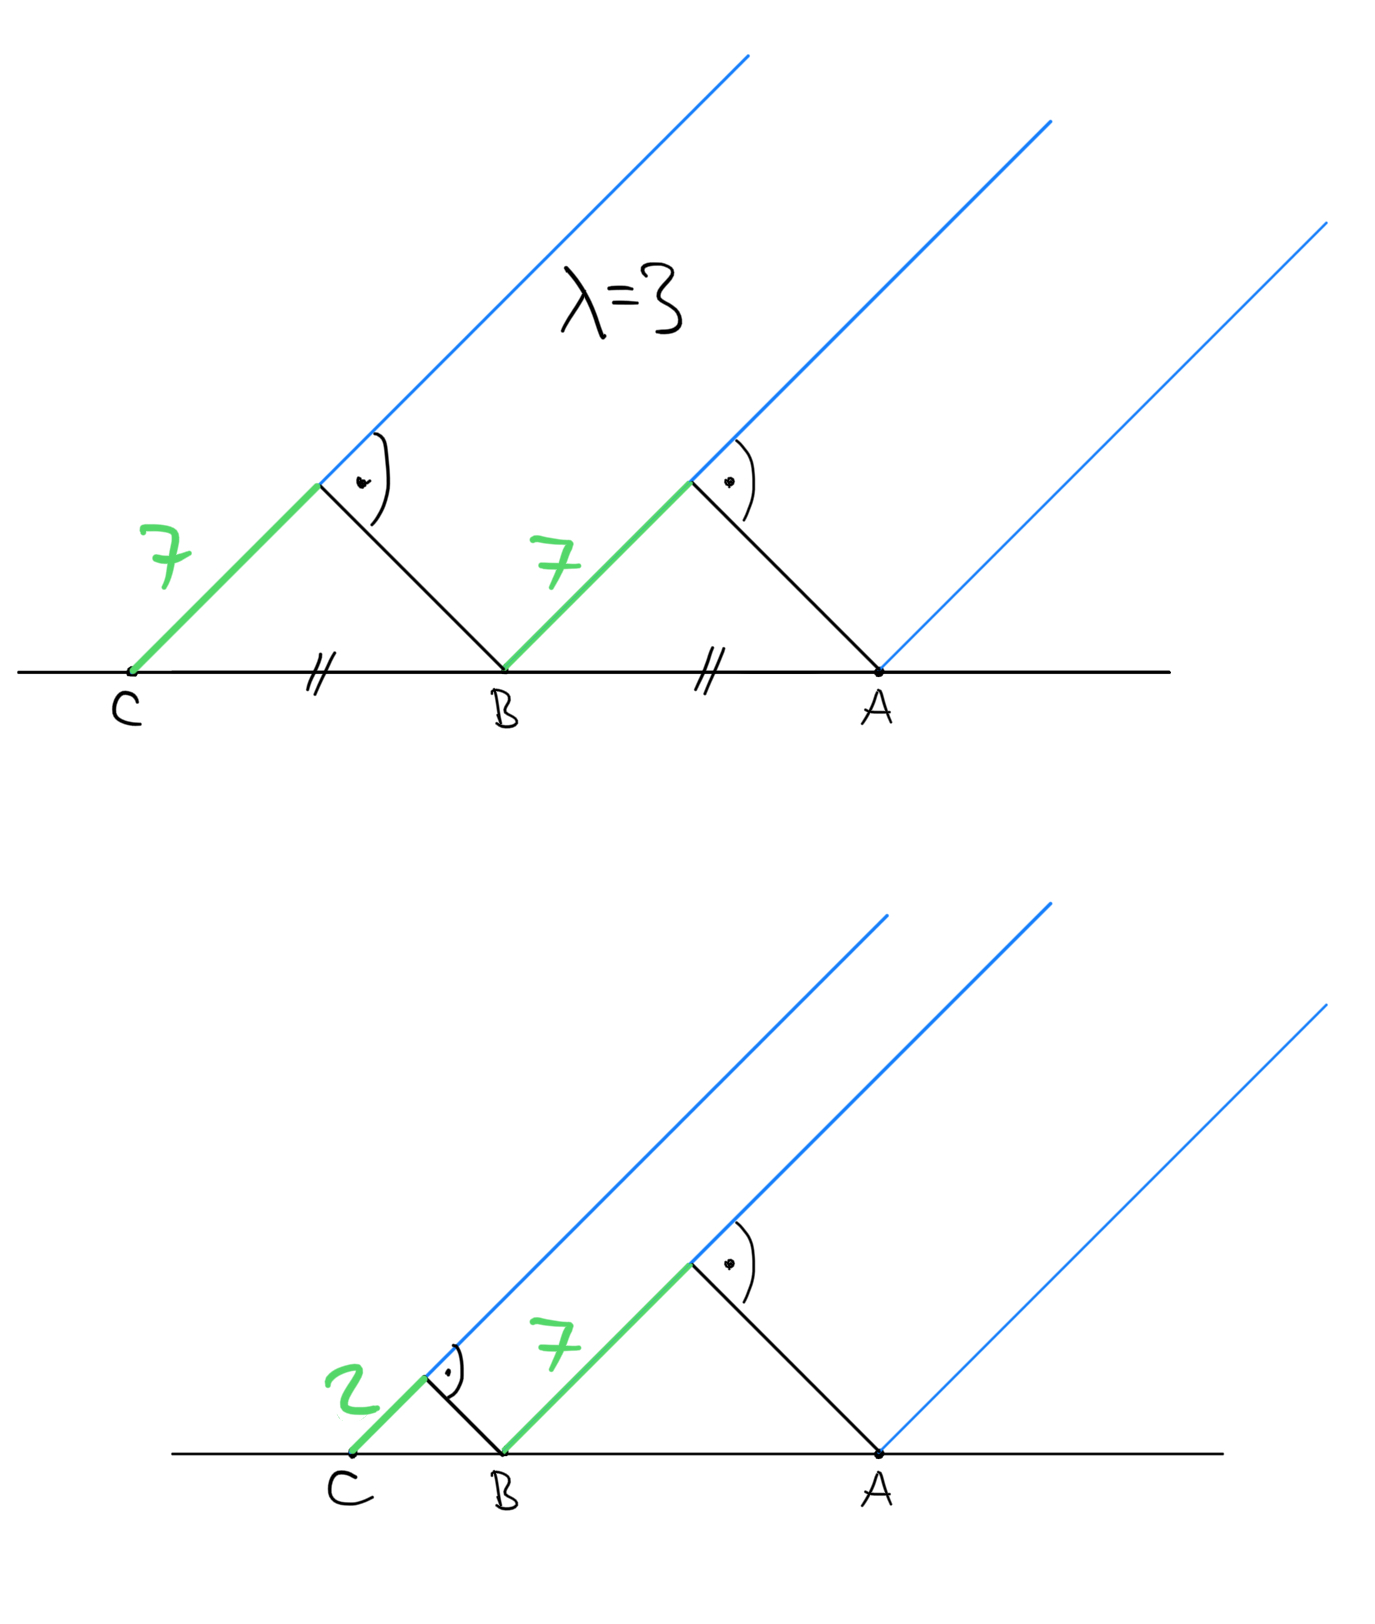
\includegraphics[width=0.4\textwidth]{k4.2/baselineunterschied.png}
  \caption{Gangdifferenzen von Radiowellen bei Antennenarrays}
  \label{k4.2.radioastro.interfero.bild.baselineunterschied}
\end{figure}

Radiointerferometrie ist ein Verfahren zur Überlagerung von Radiowellen, welche von mehreren Antennen aufgezeichnet wurden, um hieraus ein Signal zu erzeugen. Dieses Signal soll dem Signal, welches von einer Antenne mit dem Spiegeldurchmesser entsprechend des Antennenabstandes erzeugt worden wäre, möglichst ähnlich sehen.

Werden mehrere Teleskope in einem Verbund synchronisiert, ist nur die Laufzeitdifferenz im Vergleich zum Wellenberg bekannt, da die einzelnen Wellenberge nicht unterschieden werden können. So können, wie im Beispiel  \cref{k4.2.radioastro.interfero.bild.baselineunterschied}, bei gleichen Abständen nicht zwischen den Gangdifferenzen $mod \lambda$ unterschieden werden. In diesem Beispiel ist aus den Messwerten nicht ersichtlich, ob es sich tatsächlich um $2\cdot \lambda +1$ Gangunterschied handelt, sondern jedes $x$ in $x\cdot\lambda+1$ ist möglich. Werden Antennen mit unterschiedlichen Abständen verwendet, sinkt die Anzahl der Kombinationen der Gangunterschiede, für welche sich eine solche Gleichung lösen lässt. Daher werden bei Antennengruppen möglichst unterschiedliche Abstände verwendet.

Dieses Verfahren wurde beispielsweise auch \emph{Event Horizon Telescope} verwendet. Das \emph{Event Horizon Telescope} besteht aus einer Verschaltung mehrerer Teleskope, wobei deren Abstand bis zu $10000km$ beträgt. Mit diesem Teleskop wurde das erste Foto eines Schwarzen Lochs erstellt.

Die Radiointerferometrie ist also ein essenzieller Bestandteil der Astronomie. Nur dieses Verfahren ermöglicht die Ursprungsbestimmung eines Radiowellen Signals.

\subsection{Zusammenfassung}
Die Radioastronomie erstellt mithilfe von Teleskopen und Antennenarrays Bilder des Weltraums. Die Radiointerferometrie verarbeitet das Signal der Teleskope in Bilder.

\section{Pytest}
\sectionauthor{Finia Hoffman}
Pytest ist ein Testing-Framework für Python. Dabei wird die Fehlerbehebung und allgemeine Testphase der Entwicklung automatisiert und somit effizienter als manuelles Testen. Anstatt sich an ausgewählten Stellen Werte ausgeben zu lassen und diese zu überprüfen, kann man einige Test-Methoden anwenden, um so komplexere Fehler zu beheben. Pytest überprüft synthetische Eingaben für die zu testende Funktion und vergleicht die Ausgabe mit der Erwartung.

Dabei ist eine einfache Abfrage:

\begin{verbatim}
assert name_Funktion ({Eingabe}) == {gewünschte Ausgabe}
\end{verbatim}
In einem konkreten Beispiel der Addition mit 2 kännte dies wie folgt aussehen:
\begin{verbatim}
assert add_2(1) == 3
\end{verbatim}
Pytest bearbeitet nun die Methode mit den eingegebenen Werten und überprüft selbstständig die Ausgabe. Sollte die erwartete Ausgabe nicht mit der tatsächlichen übereinstimmen wird eine Fehlermeldung angezeigt. Bei automatisierter, zufälliger Testung wird zudem angezeigt, welche Eingabe und Code-Zeile zur Fehlermeldung geführt haben.

Die zu testende Methode beginnt mit 'test\_'.

Mit dem Dekorator '@pytest.fixture' vor einer Funktion lässt sich die Eingabe von zu testenden Methoden global definieren und dessen Spezifikationen automatisieren.

So können z.B. Eingabewerte zufällig generiert werden.

Auch kann man bewusst Parameter eingeben, bei denen man eine Fehlermeldung erwartet. Dabei handelt es sich um eine Überprüfung, ob falsche Eingaben wirklich als Fehler erkannt werden. Dafür gibt es den Befehl:
\begin{verbatim}
with pytest.rises({FehlerTyp})
\end{verbatim}
mit dem überprüft wird, dass die Funktion wirklich die erwartete Fehlermeldung zurückgibt.

Zuletzt kann man noch mit einer Test-Methode durch den Dekorator
\begin{verbatim}
@pytest.mark.parametrize({Eingabe})
\end{verbatim}
kennzeichnen. Hierbei werden einige charakteristisch Eingaben ausprobiert.

Wenn die automatisierten Test-Methoden ohne Fehlermeldung durchlaufen, so ist der Algorithmus scheinbar fehlerfrei. Dabei können Fehler aber nicht vollständig ausgeschlossen werden, da die Testung immer nur so gut ist wie die Ideen-Vielfalt zu potenziellen Fehlerquellen. Nicht bekannte, ungetestete Fehler können nicht vermieden werden.

\section{Fourier-Transformation}
\sectionauthor{Natalie Teplitska, Ole Fleck, Constantin Burmeister}

% Bei der Fourier-Transformation handelt es sich um eine mathematische Methode zur †bersetzung eines Signals in ein Frequenzspektrum. Aufgrund vieler unterschiedlichere Varianten findet sie sowohl Anwendung in mathematischen Bereichen, aber auch in der Physik, wie beispielsweise in unserem Kurs bei der Verarbeitung von Radiosignalen.

\begin{figure}
  \centering
  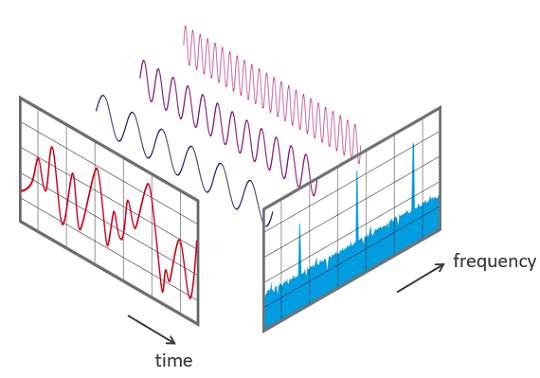
\includegraphics[width=0.6\textwidth]{k4.2/fourier.png}
  \caption{Anschauliche Darstellung der Fourier-Transformation (Quelle: \url{www.nti-audio.com})}
\end{figure}

Ein häufiges Beispiel ist die Spektralanalyse von Schallwellen. Die Daten (in der Abbildung links), die man beispielsweise mit einem Mikrofon aufnimmt, bestehen aus Schallwellen unterschiedlicher Wellenlängen. Mithilfe der Fourier-Transformation wird das Signal auf Schwingungen mit verschiedenen Wellenl\"angen aufgeteilt (in der Abbildung rechts), wodurch man das Frequenzspektrum erhält.

Abhängig von der Art der Rohdaten und der gewünschten Ausgabe finden verschiedene Varianten der Fourier-Transformation Anwendung.

Die kontinuierliche Fourier-Transformation (FT) bestätigt als Eingabe eine Funktion, über die mit $\mathcal{F}(x)(s)=\int_{-\infty}^{\infty}e^{-ist}x(t)dt$ integriert wird. Diese Berechnung lässt sich nur auf kontinuierliche Werte anwenden und gibt eine kontinuierliche Funktion aus.

Die diskrete Fourier-Transformation (DFT) kommt mit diskreten Werten aus und ist daher am Besten für digitale Signalverarbeitung geeignet, da Computer grundsätzlich mit einzelnen Datenpunkten und nicht mit kontinuierlichen Werten arbeiten. Die Formel dazu ist entsprechend kein Integral, sondern eine Summe aller gegebenen Datenpunkte: $\hat a_k = \sum\limits_{j=0}^{N-1}e^{-2\pi i\cdot\frac{jk}{N}}\cdot a_j$. Da die Laufzeit der DFT quadratisch ist, wurde die Fast Fourier Transformation (FFT) entwickelt, welche mithilfe des \emph{Divide and Conquer} (Teile-und-Herrsche) Prinzips in der Lage ist, die Rechenzeit drastisch zu reduzieren.

Manche Probleme, welche im Wertebereich nur durch viele komplizierte Operationen l\"osbar sind, k\"onnen im Bildbereich mit wenigen einfachen Operationen gel\"ost werden. Dazu transformiert man die Daten, führt die notwendigen Operationen im Bildbereich aus und transformiert die Lösung zurück in den Wertebereich. Mächte man beispielsweise eine Tonaufnahme von Störsignalen bereinigen, wendet man die FFT an, bearbeitet das Frequenzspektrum im Bildbereich und übersetzt es zurück in Musik oder Sprache. Diese Aufgabe w\"are im Wertebereich erheblich rechenintensiver gewesen.

Das \enquote{Rückübersetzen} der Signale erfolgt mit der inversen (kontinuierlichen oder diskreten) Fourier-Transformation (IFT). Diese erzeugt die Funktion, welche aus einem gegebenen Spektrum entsteht. Dazu werden dieselben Operationen wie bei der Berechnung des Spektrums rückwärts angewandt.

\section{Komplexe Zahlen}
\sectionauthor{Natalie Teplitska, Ole Fleck, Mara Germann}

Da bei der Radioastronomie komplexe Zahlen eine Rolle spielen, hat sich unser Kurs auch mit diesen beschäftigt.

Die Menge $\mathbb{C}$ ist die Menge aller Zahlen $z=a+b\cdot i$. Dabei wird $a$ als Realteil und $b$ als Imaginärteil bezeichnet. Weiterhin ist $i$ die imagin\"are Einheit mit $i^{2} = -1$. Ist $b = 0$, fällt der Imaginärteil weg und wir erhalten die bereits bekannten reellen Zahlen. $\mathbb{C}$ ist somit die Menge aus $\mathbb{R}$ und den imaginären Zahlen.

Die konjugierte komplexe Zahl von $z=a+b\cdot i$ ist definiert über $\bar{z}=a-b\cdot i$. Das Produkt aus $z$ und $\bar{z}$ hat die Eigenschaft, dass $z\cdot \bar{z}=(a+b\cdot i)\cdot (a-b\cdot i)=a^2-b\cdot i^2=a^2+b^2$ eine reelle Zahl ist.

Bei der Addition und Subtraktion von komplexen Zahlen gibt es keine Besonderheiten zu beachten, die imaginäre Einheit i wird wie eine Konstante mitgenommen. Auch die Multiplikation verläuft wie gewohnt, nur sollte man stets daran denken, dass $i\cdot i=-1$.
Die Division von komplexen Zahlen gestaltet sich etwas komplizierter, v. a. weil das Kürzen des Bruches meist nicht ohne Weiteres möglich ist. Oft hilft es aber, mit der konjugierten komplexen Zahl des Nenners zu erweitern, sodass im Nenner kein Imaginärteil mehr vorkommt und der Ausdruck erheblich vereinfacht wird. Mit diesem Wissen ist es uns möglich, mathematische Operationen auf die komplexen Zahlen anzuwenden.

Die Menge $\mathbb{C}$ lässt sich geometrisch in einem kartesischen Koordinatensystem darstellen, wobei die x-Achse für a und die y-Achse für b steht. Jede komplexe Zahl $z=a+b\cdot i$ entspricht dann genau einem Vektor $\begin{pmatrix} a \\b
  \end{pmatrix}$.
Bisher haben wir mit den komplexen Zahlen in kartesischen Koordinaten gerechnet. Sie lassen sich aber auch als Polarform angeben:
\begin{equation}
  z=r\cdot e^{i\cdot\phi}.
\end{equation}
Viele Operationen mit Vektoren kann man so viel einfacher ausführen. Dabei ist $\phi$ der Winkel des Vektors zur x-Achse und r seine Länge. Eine konjugierte komplexe Zahl ist äquivalent zur Spiegelung des Vektors an der reellen Achse.

\section{Git}
\sectionauthor{Jonas Fiedler}
Mit der Versionsmanagement-Software Git kann Kooperation zwischen mehreren Programmierern ermöglicht werden. Git beschäftigt sich hauptsächlich mit dem Verwalten der Versionen des Codes und der Zusammenführung von überlappendem Code. Dafür erstellt Git einen Versionsverlauf, welcher es ermöglicht, Versionen des Codes zurückrollen um Bugs zu identifizieren und das Nachverfolgen von Code-Änderungen von wichtigen Updates zu ermöglichen. Dabei wird zwischen lokaler Dateispeicherung und Speicherung im serverseitigen Bereich unterschieden. Der Server ermöglicht den Nutzern, Code herunterzuladen, ihn zu bearbeiten und letztendlich in überarbeiteter Version wieder an den Server zu übermitteln, wo er mit dem restlichen Code vereint wird.

Generell ist es in Git möglich verschiedene Versionsstränge (Branches) aufzubauen. Diese Branches ermöglichen die Modifikation an verschiedenen Bereichen und ein strukturiertes Arbeiten. In diesen Branches können somit bspw. Bugs unabhängig gelöst werden und neue Funktionen getestet sowie implementiert werden. Sobald diese ordnungsgemäß funktionieren, werden sie auf den nächst höheren Branch geschoben (Merge) und somit mit dem Rest des Codes wieder vereint.

In Git gibt es verschiedene Stadien, der \enquote{Codeverarbeitung} um eine Codeversion zu speichern. Dabei beschreibt Git Add den Vorgang wo die Datei von dem Working-Directory (lokal), in die Staging Area (auch lokal) verschoben wird. Das wichtigste in Git ist der Commit, dieser hält den aktuellen Zustand des gesamten Projektes fest und speichert diesen im Localrepo. Danach ermöglicht Git Push das Übertragen des Codes an den Server. Der Umkehrschritt dazu ist Git Pull. Dies lädt die aktuellste Version des Projektes vom Remoterepo in das Localrepo des Users.

Aufgrund der diversen Verwaltungsoptionen und der Möglichkeit kollaborativ in Git zu arbeiten, wird dieses Tool deshalb von äußerst vielen Programmierern verwendet.

\section{Computertomographie}
\sectionauthor{Aaron Gschwendt}

\subsection{Tomographie}

Die Tomographie ist ein bildgebendes Verfahren, in dem ein Objekt schichtweise untersucht wird. Um diese Schichten zu bestimmen, beobachtet man Strahlen, die durch das Objekt in einer Ebene gehen. Die Menge an Licht, die auf der Strecke absorbiert wurde, entspricht dem Linienintegral:

$$d=\int_{\Gamma}{}s(p)dp(\gamma)$$

$$p\in \mathbb{R}^2$$

$d$ ist hier die Menge an Licht die zwischen dem Sender und dem Empfänger absorbiert wird und wird experimentell bestimmt. Gesucht ist $s(p)$, die die optische Dichte von jedem Punkt in der Ebene darstellt. Die Gleichung lässt sich nicht analytisch bestimmen. Kennt man jedoch $d$ von vielen Strecken im Bild, kann man mithilfe vom bayesschen Verfahren mit hoher Auflösung und Sicherheit $s(p)$ bestimmen.

\subsection{Astronomie}

In der Astronomie wird die Tomographie verwendet, um die Form von kosmischen Wolken zu ermitteln. Dafür werden Sterne, deren absolute Helligkeit und Distanz man kennt und um bzw. in der Wolke liegen beobachtet. Man vergleicht deren scheinbare Helligkeit mit deren zu erwartende Helligkeit und ermittelt so $d$ für alle Strecken zwischen der Erde und den beobachteten Sternen. Daraus kann man $s(p)$ abschätzen und Aussagen über die dichte-Verteilung und Form der Wolke treffen

\subsection{CT}

Häufig verwendet wird die Tomographie auch in der Medizin, bekannt als Computertomographie, kurz CT.

Bei herkömmlichen Röntgenuntersuchungen werden Röntgenstrahlung durch das abzubildende Objekt auf einen Röntgenfilm oder einer Sensorplatte geleitet. Das 3d-Objekt wird dabei auf eine 2d-Fläche projektiert. Der Nachteil dieser Methode ist das sich Teile vom Objekt überlagern können und man nicht erkennen kann, ob es sich um ein Objekt mit hoher Absorption oder mehrere Objekte mit geringer Absorption handelt.

Beim CT drehen sich im $180^\circ$ Winkel eine Röntgenröhre und Detektor um den Patienten und nimmt dabei in kleinen Abständen Messpunkte auf. Dieses wird für einige Schichten entlang des zu untersuchenden Körperteils ausgeführt. Der Röntgenstrahl ist breit genug damit bei jedem Messpunkt die ganze breite des Körperteils in einem Streifen ergriffen wird aber sehr dünn, um die vertikale Auflösung zu erhöhen.

\begin{wrapfigure}{r}{0.4\linewidth}
  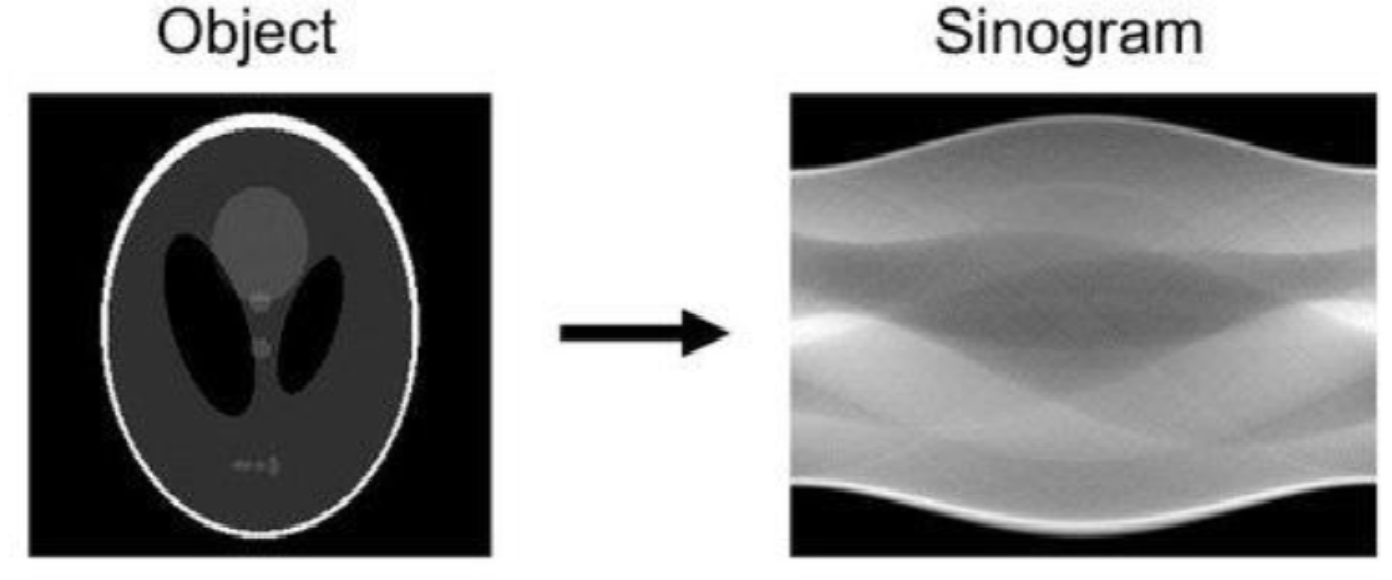
\includegraphics[width=0.4\textwidth]{k4.2/backprojektion.png}
  \caption{Sinogram}
  \label{k4.2.tomo.ct.bp}
\end{wrapfigure}

Daraus entsteht für jede Schicht ein Sinogram \cref{k4.2.tomo.ct.bp} bei der eine Achse (hier Y-Achse) das Absorptionsprofil und die andere (hier X-Achse) dem Winkel entspricht. Jede Stelle im Objekt bildet eine Sinuskurve; ihr Abstand vom Mittelpunkt entspricht der Amplitude und ihr Winkel im vergleich zum Startpunkt der Phasenverschiebung der Sinuskurve. Mit dem bayeschen Verfahren  kann man ein Bild von der Schicht mit hoher Genauigkeit rekonstruieren. Macht man dies für jede Schicht erhält man ein 3d-Rendering des Objekts.

\section{NumPy}\label{k4.2.ch.NumPy}
\sectionauthor{Cedric Balzer}
Numerisches Python (kurz. Numpy) ist ein auf in der Programmiersprache geschriebene Libary für Python. Sie ermöglicht das effiziente Rechnen mit Matrizen, mehrdimensionalen Arrays und Vektoren in Python.

NumPy ist eine open-source Library welche auf den früheren Python-Modulen Numeric und Numarray basiert. Da Python nicht für numerische Rechnung optimiert ist, greift NumPy auf den schnelleren C Compiler zurück und ermöglicht damit das numerische Rechnen auch mit großen Datenmengen. Eine der Kernfunktionalitäten von NumPy ist das mehrdimensionale Array, das eine Matrix von Elementen repräsentieren kann. Ein zentraler Unterschied im Vergleich zu Python-Listen ist, dass alle im Array gespeicherte Elemente vom selben Datentyp sein müssen. Außerdem ist die Größe eines NumPy-Arrays statisch und jedes Element im Array muss einen Wert enthalten, sodass keine leeren Eintrage im Array erstehen. Dies liefert eine im Vergleich zu Listen eine schnellere Handhabung.
Numpy ist nicht im Python3-Standard enthalten und muss daher separat installiert werden:

\begin{verbatim}
pip install numpy
\end{verbatim}

Möchte man ein Array aus einer Liste erstellen bietet sich folgender Code an:

\begin{verbatim}
>>> import numpy as np
>>> nums = [1,2,3,4,5]
>>> a = np.array(nums)
>>> a
array([1, 2, 3, 4, 5])
\end{verbatim}

Besteht eine übergebene Liste aus mehreren Teillisten wird ein mehrdimensionales Array erstellt:

\begin{verbatim}
>>> import numpy as np
>>> m1 = np.array([ [1,2,3], [4,5,6], [7,8,9] ])
>>> m1
array([[1,2,3],
       [4,5,6],
       [7,8,9]])
\end{verbatim}

Möchte man auf ein Element eines eindimensionalen Arrays zugreifen, so funktioniert dies wie bei Listen. Um in mehrdimensionalen Numpy-Arrays Werte zu selektieren, wird folgende Syntax verwendet:

\begin{verbatim}
>>> import numpy as np
>>> a = np.array([1,2,3,4,5,])
>>> a[3]
4

>>> a[-1]
5
\end{verbatim}

Auf Arrays können einfache Rechenoperatoren, wie Plus und Minus, angewandt werden. Diese Rechnungen werden elementweise ausgeführt, es werden stets neue Arrays erzeugt und die Original-Arrays bleiben unverändert.

\begin{verbatim}
>>> import numpy as np
>>> r = np.arange(10)
>>> r
array([0, 1, 2, 3, 4, 5, 6, 7, 8, 9])

>>> r+1
array([1, 2, 3, 4, 5, 6, 7, 8, 9, 10])

>>> r**2
array([0, 1, 4, 9, 16, 25, 36, 49, 64, 81])
\end{verbatim}

Des Weiteren gibt es in Numpy Operationen speziell für Matrizen und Vektoren.
Für Matrix-Arrays existieren zusätzlich die Numpy-Funktionen \verb|dot()|, \verb|inner()| und \verb|outer()|, mit deren Hilfe Multiplikationen von Matrizen beziehungsweise Vektoren durchgeführt werden können (siehe \cref{k4.2.ch.linalg}).

\begin{verbatim}
>>> import numpy as np
>>> a = [[1, 0], [0, 1]]
>>> b = [[4, 1], [2, 2]]
>>> np.dot(a, b)
array([[4, 1],
       [2, 2]])
\end{verbatim}

Neben \verb|dot()| liefert NumPy den \verb|@| Operator (\verb|np.matmul()|) welcher ebenfalls Arrays und Matrizen multiplizieren kann.
Bei einer Multiplikation von Vektoren und 2D Matrizen erzeugen diese Funktionen identischen Output:

\begin{itemize}
\item Skalarmultiplikation zweier Vektoren
\begin{verbatim}
>>> import numpy as np
>>> a = np.array([1,2])
>>> b = np.array([2,2])
>>> np.dot(a,b)
6

>>> a@b
6
\end{verbatim}

\item Multiplikatipon zweier Matrizen
\begin{verbatim}
>>> import numpy as np
>>> a = np.array([[1,2],[5,3]])
>>> b = np.array([[2,2],[8,1]])
>>> np.dot(a,b)
array([[18  4]
       [34 13]])

>>> a@b
array([[18  4]
       [34 13]])
\end{verbatim}
\end{itemize}

Numpy ist ein nützliches und effizientes Tool, um mit großen Datenmengen zu arbeiten. Es liefert durch diese umfassende Funktionalität die Grundlagen für andere wissenschaftlich genutzten Libaries.

\section{Objekt-Orientierte Programmierung}
\sectionauthor{Alexander Gitnik, Clemens Ljungh}
Die Objekt-Orientierte Programmierung ist der heute am weitesten verbreitete Programmierstil. Beim Objekt-Orientierten Programmieren ist das ausschlaggebende Kriterium, dass man den Code in sinnvolle Bausteine zerlegt - dies bedeutet konkret, dass man Klassen erstellt, welche oftmals reale Objekte darstellen.

Dabei ist eine Klasse eine allgemeine Vorlage, aus der einzelne Objekte, die \emph{Klasseninstanzen}, initialisiert werden können. Folglich besitzen genannte Klassen zum einen Eigenschaften, \emph{Attribute} genannt, und zum anderen Handlungsmöglichkeiten, welche \emph{Methoden} genannt werden. Jede Klasse besitzt einen Konstruktor, welcher bei jeder Erstellung einer \emph{Instanz} der Klasse automatisch aufgerufen wird, und an welchen gegebenenfalls auch die zum Erstellen einer Klasse benötigten Anfangsparameter übergeben werden. Objekte initialisiert man durch Zuweisung des Konstruktoraufrufs der jeweiligen Klasse an eine Variable, welche nun zu einem Objekt des Klassentyps wird. Da es vorkommt, dass sich Klassen ähneln, kann man \emph{Attribute} und \emph{Methoden} von einer \emph{Superklasse} an eine \emph{Unterklasse} vererben, sodass all jener Klasseninhalt an die \emph{Unterklasse} weitergegeben wird.

Allgemein gilt bei der Objekt-Orientierten Programmierung die Konvention, dass \emph{Attribute} lediglich über \emph{Getter- und Setter-Methoden} abgefragt und verändert werden. Dies hat den Grund, dass man nicht versehentlich einen Fehler in den inneren Zustand des Objekts einbaut. Nutzt man nämlich eine \emph{Settermethode}, kann man überprüfen welche Werte ein Attribut annimmt. Weiterhin existiert regulär auch die Limitation des ausschließlichen Aufrufs eines beliebigen Klasseninhalts über eine bereits initialisierte Instanz jener Klasse, welche jedoch durch Nutzung eines Dekorators, der die Methode statisch macht, aufgehoben werden kann, sodass eine Mathode über die allgemeine Klasse aufgerufen werden kann.

\section{Funktionale Programmierung}
\sectionauthor{Alexander Gitnik, Clemens Ljungh}
Die Funktionale Programmierung ist ein gänzlich anderes Konzept als die Objekt-Orientierte Programmierung. Ihren Ursprung hat die Funktionale Programmierung im Lambda-Kalkül. Das Lambda-Kalkül kommt aus der Mathematik und ist eine formale Sprache, um logische Systeme darzustellen. Außerdem ist das Lambda-Kalkül Turing-vollständig, dies bedeutet, dass man jedes Programm damit ausdrücken kann.

Anders als bei der Objekt-Orientiertem Programmierung werden Daten bei der Funktionalen Programmierung nicht in Objekten gespeichert, sondern hauptsächlich über einzelne Funktionen ausgewertet. Diese Funktionen müssen dabei \emph{pur} sein. \emph{Pure Funktionen} ähneln mathematischen Funktionen: Sie geben bei gleicher Eingabe immer die gleiche Ausgabe, da sie keinen inneren Zustand haben, welcher die Eingabe manipulieren oder verändern könnte. Weiterhin ändern die puren Funktionen auch nichts außerhalb der eigenen Funktion

Üblich ist es auch, dass Funktionen als Parameter eine weitere Funktion entgegennehmen können, sodass jene über ihre Rückgabewerte ineinander verschachtelt werden. Dies endet darin, dass bei der Funktionalen Programmierung eine Kette aus Befehlen entstehen kann. Häufig wird in der Funktionalen Programmierung die \emph{Rekursion} verwendet, was bedeutet, dass Funktionen sich selber aufrufen können.

Daten sind bei der Objekt-Orientierten Programmierung zwar besser strukturiert, dafür sind gerade die puren Funktionen der Funktionalen Programmierung einfacher für Entwickler zu verstehen, da die puren Funktionen keinen komplexen inneren Zustand haben. Wichtig für die Funktionale Programmierung ist das Konzept der \emph{Lazy Evaluations}. Dies bedeutet, dass Ausdrücke, welche nicht direkt für das Endergebnis benötigt werden gar nicht erst ausgerechnet werden oder zumindest erst wenn sie gebraucht werden. Dadurch kann die Laufzeit eines Programmes verringert werden, was vorteilhaft ist.

Heutzutage ist die Funktionale Programmierung weitestgehend von der Objekt-Orientierten Programmierung verdrängt worden. Für unsere Kursarbeit brauchen wir oft die Funktionale Programmierung, da wir Datensätze rein mathematisch verarbeiten. Außerdem ist Python gut für die Funktionale Programmierung geeignet.

\section{Conjugate Gradient/Gradient Decent - LGS-Lösungsalgorithmen}
\sectionauthor{Benjamin Knöbel del Olmo, Leo Bergmann}

Wie in der Betrachtung von eindimensionalen Funktionen, werden für die Bestimmung der Extrema auch bei mehrdimensionalen Funktionen Ableitungen eingesetzt. Diese werden nicht mehr durch reelle Zahlen, sondern durch Vektoren ausgedrückt. Gegeben sei die eine differenzierbare Funktion $ f:\mathbb{R}^n \rightarrow \mathbb{R}, x \rightarrow f(x). $ Die Ableitung von f an einem Punkt entspricht einem N-Dimensionalen Vektor. Dieser heißt Gradient und seine Spitze zeigt immer in Richtung des stärksten Anstiegs, wobei dessen Länge der Steigung entspricht.

Darauf basiert der Gradient Descent Algorithmus, der das Ziel hat, das Minimum einer Funktion, also den Punkt, an dem $ f'(x) = 0 $ gilt, zu finden. Dies wird durch einen iterativen Ansatz erreicht: An einem zufällig gewählten Startpunkt wird zunächst der Gradient ermittelt. Danach wird als neuen Startpunkt derjenige definiert, der durch das Gehen in die entgegengesetzte Richtung des Gradienten erreicht wird. Die Länge des gegangenen Schrittes hängt von der Länge des Gradienten ab, die durch eine Konstante, die Learning Rate, skaliert wird. Der Algorithmus endet, wenn die davor definierte, maximale Anzahl an Durchläufen erreicht, oder wenn die Schrittlänge kleiner als eine davor definierte Toleranz ist. Der Gradient Descent ist also ein Näherungs-/Optimierungsalgorithmus.

Vorausgesetzt wird, dass die Funktion differenzierbar und konvex ist, also ein Minimum besitzt. Auch Funktionen mit Sattelpunkt oder Durchführungen mit unpassenden Learning Rates können zu falschen Ergebnissen und langen Laufzeiten führen. Das liegt daran, dass bei zu großen Learning Rates das Minimum einfach übergangen wird, während bei zu kleinen Learning Rates der Algorithmus in kleinesten lokalen Minima „stecken“ bleibt, wobei das Programm dann ohne Fortschritt weiterläuft.

Um das zu verhindert existiert für lineare Funktionen ein weiterer Algorithmus namens Conjugate Gradient. Auch er basiert auf der Minimabestimmung, um ein lineares Gleichungssystem (LGS) zu lösen.

Ein LGS wird durch die Formel $A\vec{x} = \vec{b}$ dargestellt, wobei A eine $ n \times n $-Matrix (invariant unter Transposition) und $ b,x $ Vektoren sind und kann durch die Ableitung gelöst werden. Das geht, indem eine quadratische Funktion nach dem Schema $ f(x) = 1/2xAx-bx+c $ notiert wird, (mit selben A,b und x), dessen komponentenweise Ableitung genau dann null ist, wenn das ursprüngliche lineare Gleichungssystem nach x gelöst ist, da gilt: $f'(x) = Ax-b = 0$. Daher ist das Optimieren der dem LGS entsprechenden Funktion äquivalent zum Lösen ebenjenes.

Algorithmisch: Conjugate Gradient läuft das Residuum (welches der Vektor ist, der entgegengesetzt zum oben erwähnten Gradienten, also additiv invers verläuft) ab, aber korrigiert die „Abstiegsrichtung“ in Betrachtung aller vorher gegangenen Residuen so, dass diese A-orthogonal (engl. conjugate) zu allen vorherigen ist. Daraus folgt, dass wir nach maximal n-Schritten am Ziel ankommen, da wir dann alle n Dimensionen der $ n \times n $-Matrix optimal abgegangen sind. Der Algorithmus hat also zwei Endbedingungen, zum einen, wenn n Iterationen erreicht sind, oder wenn die Differenz zum Endergebnis, also das $ f'(x) = 0 $ gilt, klein genug ist.
Gradient Descent und Conjugate Gradient ermöglicht es uns also, lineare Gleichungssysteme zu lösen und dadurch Daten, die in Matrizen gespeichert sind, weiterzuverarbeiten. Ein Beispiel wäre die Lösung der Gleichung  $ D^{-1} m = j $, auf die im Kapitel \enquote{Wiener Filter} eingegangen wird.

% Bibliography
\printbibliography{}
\end{document}
